% Preamble
\documentclass[10pt, letterpaper]{article}
%\usepackage[T1]{fontenc}
\usepackage{graphicx}
\usepackage{amsmath}

% Packages - bibliography management
\usepackage[backend=biber,style=nature]{biblatex}
\addbibresource{bib/refs_LDCV.bib}
%\DeclareFieldFormat{labelnumberwidth}{}
%\setlength{\biblabelsep}{0pt}

% Header
\title{Lid-Driven Cavity Flow: A Finite-Volume Implementation}
\date{}
\author{Jay V. Evans}

% Document
\begin{document}
\maketitle

\section{Problem Description}

\begin{figure}[h]
    \centering
    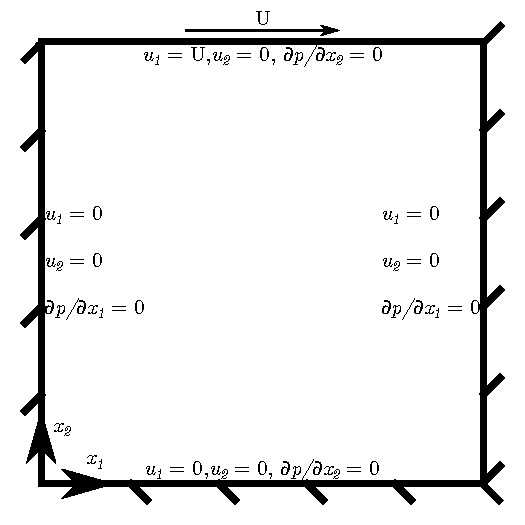
\includegraphics[]{img/problem.pdf}
    \caption{Lid-driven cavity flow problem illustration.}
    \label{fig:problem}
\end{figure}


\section{Governing Equations}

\subsection{Differential Equations}

The form of the incompressible Navier-Stokes equations, and their subsequent non-dimensionalization are taken from Ferziger and Perić \cite{Ferziger_Springer_2002}. Dimensional quantities are shown with a ``*'' superscript, and non-dimensional quantities are shown without modification. Conservation of mass, with dimensional units is shown in Eq. \ref{eq:cont_dim}. Similarly, the dimensional form of the momentum equation is given in Eq. \ref{eq:mom_dim}.

\begin{equation}
  \frac{\partial{u_{i}^{*}}}{\partial{x_{i}^{*}}} = 0
  \label{eq:cont_dim}
\end{equation}

\begin{equation}
  \frac{\partial{u_{i}^{*}}}{\partial{t^{*}}} + \frac{\partial{(u_{j}^{*}}u_{i}^{*})}{\partial{x_{j}^{*}}} ={\nu^{*}}\frac{\partial^{2}{u_{i}^{*}}}{\partial{x_{j}^{2}}} - \frac{1}{\rho^{*}}\frac{\partial{p^{*}}}{\partial{x_{i}^{*}}}
  \label{eq:mom_dim}
\end{equation}

The dimensional quantities of Eq. \ref{eq:cont_dim}, \ref{eq:mom_dim}, are nondimensionalized according to Eqs. \ref{eq:time_ndim} - \ref{eq:press_ndim}.

\begin{equation}
  t = \frac{t^{*}}{t_{0}^{*}}
  \label{eq:time_ndim}
\end{equation}


\begin{equation}
  x_{i} = \frac{x_{i}^{*}}{L_{0}^{*}}
  \label{eq:dist_ndim}
\end{equation}


\begin{equation}
  u_{i}^{*} = \frac{u_{i}^{*}}{v_{0}^{*}}
  \label{eq:vel_ndim}
\end{equation}


\begin{equation}
  p = \frac{p^{*}}{\rho^{*}v_{0}^{*2}}
  \label{eq:press_ndim}
\end{equation}

Accordingly, the nondimensional form of the continuity and momentum equation are shown in Eq. \ref{eq:cont_ndim} and \ref{eq:mom_ndim}, respectively. In these equations, $L_{0}^{*}$ is the reference length dimension, $t_{0}^{*}$ is the reference time dimension, $v_{0}^{*}$ is the refence velocity dimension, and $\rho^{*}$ is the density of the fluid.

\begin{equation}
  \frac{\partial{u_{i}}}{\partial{x_{i}}} = 0
  \label{eq:cont_ndim}
\end{equation}

\begin{equation}
  \boxed{
  \text{St}\frac{\partial{u_{i}}}{\partial{t}} + \frac{\partial{(u_{j}u_{i})}}{\partial{x_{j}}} =\frac{1}{\text{Re}}\frac{\partial^{2}{u_{i}}}{\partial{x_{j}}} - \frac{\partial{p}}{\partial{x_{i}}}
  \label{eq:mom_ndim}
  }
\end{equation}

As a result of the nondimensionalization, the dimensionless numbers, $\text{Re}$ (Reynolds number) and $\text{St}$ (Strouhal number) appear in Eq. \ref{eq:mom_ndim}. While Eqs. \ref{eq:cont_ndim} and \ref{eq:mom_ndim} mathematically express mass and momentum conservation, respectively, with regards to implementing these numerically, the continuity equation (Eq. \ref{eq:cont_ndim}) does not provide any additional information that is not contained in the momentum equation (Eq. \ref{eq:mom_ndim}). The continuity equation must be further manipulated into a form which can be implemented to enforce mass continuity. Computing the divergence of the momentum equation (Eq. \ref{eq:mom_ndim}) yields Eq. \ref{eq:mom_ndim_div}. Simplifying Eq. \ref{eq:mom_ndim_div} produces equation Eq. \ref{eq:mom_ndim_div_simp}. Applying the contuinuity equation to Eq. \ref{eq:mom_ndim_div_simp} yeilds, Eq. \ref{eq:press_poiss}, the pressure Poisson equation. In solving the pressure Poisson equation, mass conservation is enforced. Note that there is not a fluid equation of state for closure in which \textit{absolute} pressure appears as a term. In incompressible flow, only \textit{gradients} of pressure appear in the momentum equation, thus by solving Eq. \ref{eq:press_poiss}, a pressure field which satisfies continuity is determined.

\begin{equation}
  \frac{\partial}{\partial{x_{i}}}\bigg(\text{St}\frac{\partial{u_{i}}}{\partial{t}}\bigg) + \frac{\partial}{\partial{x_{i}}}\bigg(\frac{\partial{(u_{j}u_{i})}}{\partial{x_{j}}}\bigg) =\frac{\partial}{\partial{x_{i}}}\bigg(\frac{1}{\text{Re}}\frac{\partial^{2}{u_{i}}}{\partial{x_{j}}}\bigg) -\frac{\partial}{\partial{x_{i}}}\bigg(\frac{\partial{p}}{\partial{x_{i}}}\bigg)
  \label{eq:mom_ndim_div}
\end{equation}


\begin{equation}
  \text{St}\frac{\partial}{\partial{t}}\bigg(\frac{\partial{u_{i}}}{\partial{x_{i}}}\bigg) + \frac{\partial}{\partial{x_{i}}}\bigg(\frac{\partial{(u_{j}u_{i})}}{\partial{x_{j}}}\bigg) = \frac{1}{\text{Re}}\frac{\partial}{\partial{x_{j}}}\bigg(\frac{\partial}{\partial{x_{j}}}\bigg(\frac{\partial{u_{i}}}{\partial{x_{i}}}\bigg)\bigg) -\frac{\partial}{\partial{x_{i}}}\bigg(\frac{\partial{p}}{\partial{x_{i}}}\bigg)
  \label{eq:mom_ndim_div_simp}
\end{equation}

\begin{equation}
  \boxed{
    \frac{\partial}{\partial{x_{i}}}\bigg(\frac{\partial(u_{j}u_{i})}{\partial{x_{j}}}\bigg) = - \frac{\partial}{\partial{x_{i}}}\bigg(\frac{\partial{p}}{\partial{x_{i}}}\bigg)
  }
  \label{eq:press_poiss}
\end{equation}


\subsection{Integral Equations}

The integral forms of the non-dimensional momentum equation (Eq. \ref{eq:mom_ndim}) is required to apply a finite volume method numerical solution. The integral form of the non-dimensional momentum equation is obtained by integrating the differential form of the equation over a volume domain, $\Omega$, which yields Eq. \ref{eq:mom_ndim_int_0}. Gauss's Divergence Theorem is applied to Eq. \ref{eq:mom_ndim_int_0} to transform the volume integrals over a volume domain $\Omega$ into surface integrals over a surface boundary $\sigma$. Furthermore, the constant non-dimensional terms are moved outside of the integrals, producing Eq. \ref{eq:mom_ndim_int}. This integral form of the nondimensional pressure equation, Eq. \ref{eq:mom_ndim_int} is used for solving control volume problem, and thus is intuitive for applying to the uniform two-dimensional cells of this problem. The non-dimensional pressure Poisson equation, Eq. \ref{eq:press_poiss}, is left in differential form. 

\begin{equation}
  \int_{\Omega}\text{St}\frac{\partial{u_{i}}}{\partial{t}}d\Omega + \int_{\Omega}\frac{\partial(u_{j}u_{i})}{\partial{x_{j}}}d\Omega = \int_{\Omega}\frac{1}{\text{Re}}\frac{\partial^{2}u_{i}}{\partial{x_{j}^{2}}}d\Omega - \int_{\Omega}\frac{\partial{p}}{\partial{x_{i}}}d\Omega
  \label{eq:mom_ndim_int_0}
\end{equation}

\begin{equation}
  \boxed{\text{St}\int_{\Omega}\frac{\partial{u_{i}}}{\partial{t}}d\Omega + \int_{\sigma}{u_{j}u_{i}n_{j}}d\sigma = \frac{1}{\text{Re}}\int_{\sigma}\frac{\partial{u_{i}}}{\partial{x_{j}}}n_{j}d\sigma - \int_{\sigma}{pn_{j}}d\sigma}
  \label{eq:mom_ndim_int}
\end{equation}

\section{Discretization}

\subsection{Domain and Grid}

\printbibliography{}

\end{document}


